% ====================================
% = Dossier d'Architecture Technique =
% ====================================
% Joris Berthelot <joris@berthelot.tel>
% Laurent Le Moine <laurent.le.moine17@gmail.com>
% 
% Filename: rapport.tex
% Date: Lun, 24 oct 2011 04:00:24 CEST
% Tab size: 4
% Soft tabs: YES
% Column limit: 80
% Word count: 4033

\documentclass[11pt,a4paper]{report}
\usepackage{
    content/fullpage, % Enclosed as .sty file
    hyperref,
    listings,
    lmodern,
    soul,
    fancyhdr,
    minted % How to install: http://blog.eexit.net/2011/02/latex-colorez-efficacement-votre-code-source-avec-minted.html
}
\usepackage[utf8]{inputenc}
\usepackage[T1]{fontenc}
\usepackage[french]{babel}
\usepackage[pdftex]{graphicx}
\pagestyle{fancyplain}
\fancyhf{}
\lhead{\fancyplain{}{Dossier d'Architecture Technique}}
\rhead{\fancyplain{}{Universit\'e de La Rochelle}}
\lfoot{\fancyplain{}{Joris \textsc{BERTHELOT} - Laurent \textsc{LE MOINE}}}
\rfoot{\fancyplain{}{\thepage}}
\definecolor{lightgray}{gray}{.95}
\usemintedstyle{manni}
\newminted{bash}{
    linenos=false,
    bgcolor=lightgray,
    tabsize=4,
    gobble=20,
    fontfamily=courier,
    fontsize=\small,
    xleftmargin=5pt,
    xrightmargin=5pt
}
\newminted{php}{
    linenos=false,
    bgcolor=lightgray,
    tabsize=4,
    gobble=24,
    fontfamily=courier,
    fontsize=\small,
    xleftmargin=5pt,
    xrightmargin=5pt
}
\hypersetup{
    bookmarks=true,
    unicode=true,
    pdfstartview={FitW}
    pdftitle={Dossier d'Architecture Technique},
    pdfauthor={Joris Berthelot, Laurent Le Moine},
    pdfnewwindow=true,
    colorlinks=true,
    citecolor=black,
    filecolor=black,
    linkcolor=black,
    urlcolor=black
}
\begin{document}
    \newcommand{\HRule}{\rule{\linewidth}{0.5mm}}

\begin{titlepage}

\begin{center}


% Upper part of the page

\includegraphics[width=0.15\textwidth]{content/logo.png}\\[1cm]

\textsc{\LARGE Universit\'e de La Rochelle}\\[1.5cm]

\textsc{\Large Rapport de projet}\\[0.5cm]


% Title
\HRule \\[0.4cm]
{ \huge \bfseries Dossier d'Architecture Technique}\\[0.4cm]

\HRule \\[1.5cm]

% Author and supervisor
\begin{minipage}{0.4\textwidth}
    \begin{flushleft} \large
        \emph{Auteurs:}\\
        Joris \textsc{BERTHELOT}\\
        Laurent \textsc{LE MOINE}
    \end{flushleft}
\end{minipage}
\begin{minipage}{0.4\textwidth}
    \begin{flushright} \large
        \emph{Superviseurs:} \\
        Philippe \textsc{HARRAND}\\
        Bertrand \textsc{VACHON}
    \end{flushright}
\end{minipage}

\vfill

% Bottom of the page
{Master ICONE 2011-2012}

\end{center}

\end{titlepage}
    \newpage
    \setcounter{secnumdepth}{3}
    \setcounter{tocdepth}{4}
    \tableofcontents
    \newpage
        
        \section*{Introduction}
        
        \addcontentsline{toc}{section}{Introduction}
        
        Dans le cadre de notre formation Master Ing\'eni\'erie Informatique et de son Unit\'e d'Enseignement Architecture: Conception et Gestion, nous avons r\'ealis\'e un projet d'architecture r\'eseau HA (High Availability) en 3 jours seulement.\\
        
        Ce projet nous a permis de mettre en exergue nos connaissances r\'ecemment acquises lors des cours respectifs de la m\^eme UE mais aussi de reprendre et appliquer les concepts vus en TP la semaine auparavant.
        
        \addcontentsline{toc}{section}{Postes de travail}
            
            Assign\'e comme table \no5, nous avons utilis\'e les postes suivants :\\
            
            \begin{description}
                \item[Joris Berthelot (sera la machine << JB >> dans le reste du rapport)] \hfill \\
                    \begin{itemize}
                        \item Adresse IP: 10.192.10.23
                        \item Host: mamba13
                    \end{itemize}
                \item[Laurent Le Moine (sera la machine << LLM >> dans le reste du rapport)] \hfill \\
                    \begin{itemize}
                        \item Adresse IP: 10.192.10.24
                        \item Host: mamba14
                    \end{itemize}
            \end{description}
            
        \addcontentsline{toc}{section}{Code source}
            
            Etant donn\'e que ce projet fut r\'ealis\'e en \'equipe, le code source des diff\'erents scripts et fichiers de configuration sont disponible sur Google Code + Subversion. Ainsi, vous pouvez \`a tout moment r\'ecup\'erer notre travail (ainsi que le code {\LaTeX} du document) comme ceci :\\
            
            \begin{bashcode*}{gobble=16}
                svn export http://ulr-acg.googlecode.com/svn/trunk/ ulr-acg-src
            \end{bashcode*}
            
    \part{Infrastructure logicielle}
        
        Avant toute choses, vous devez savoir que l'ensemble des op\'erations d\'ecrites dans cette section sont a r\'ealiser avec l'utilisateur root. Si vous lancez les scripts livr\'es avec le rapport sans \^etre root, vous aurez droit \`a un gentil message d'erreur.\\
        
        Nous avons aussi par ailleurs vid\'e et d\'esactiv\'e les tables de pare-feu afin de laisse toute nos applications travailler sans avoir de g\^ene dans un premier temps :\\
        
        \begin{bashcode*}{gobble=12}
            # Vide les iptables
            /sbin/chkconfig --del iptables
            # Desactive le firewall
            service iptables stop
            # Active la synchronisation du temps sur le reseau
            service ntpd start
        \end{bashcode*}
        
        \section{Installation des paquets}
            
            Avant de commencer \`a configurer et d\'eployer les services, nous aurons besoin d'installer un certain nombre de paquets afin de pouvoir parvenir \`a nos fins. Aussi divers que vari\'es, nous avons script\'e cette installation afin de faciliter la t\^ache.\\
            
            \subsection{Configuration du proxy}
                
                Il faudra auparavant configurer manuellement les param\`etres du proxy si besoin afin de ne pas rendre le script d'installation inop\'erationnel.
                Pour se faire, veillez \`a bien changer les param\`etres dans les Serveur mandataires (Syst\`eme > Configuration > Serveurs mandataires) ainsi que rajouter les bons param\`etres \`a Yum (proxy) :\\
                
                \begin{bashcode}
                    # Configuration de Yum
                    vim /etc/yum.conf
                \end{bashcode}
                
        \section{R\'eplication bas niveau}
            
            La r\'eplication bas niveau permet de cr\'eer non pas une redondance applicative mais directement sur le support des donn\'ees applicatives (syst\`eme de fichier). L'int\^eret \`a cela est d'\'eviter de configurer chaque service pour sa propre r\'eplication (si existant) et d'aller droit au but en r\'epliquant directement le volume sur lequel repose les donn\'ees.\\
            
            Voici un petit sch\'ema (issu du site de DRBD) afin d'imager le concept : \\
            
            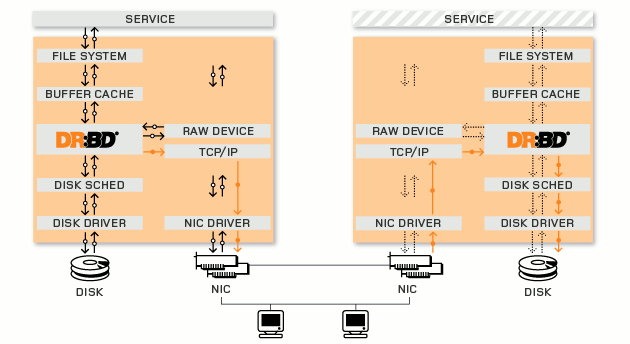
\includegraphics[keepaspectratio=true, width=\textwidth]{content/drbd.png}\\[1cm]
            
            \subsection{Installation}
                
                Pour la r\'eplication bas niveau (syst\`eme de fichiers), nous avons utilis\'e \underline{\href{http://www.drbd.org/}{DRBD}} : un logiciel permettant de faire de la r\'eplication de donn\'ees au sein d'une architecture en grappe. DRBD est assez complexe et fastidieux \`a mettre en place car il demande quelques notions assez pouss\'ees sur les volumes, leur synchronisations, etc.\\
                
                Ce logiciel ne fonctionnait autrefois qu'en mode ma\^itre/esclave mais depuis les derni\`eres versions, on peut partir sur une configuration ma\^itre/ma\^itre afin que les donn\'ees soient bien synchronis\'ees de mani\`ere bidirectionnelle.\\
                
                \begin{bashcode}
                    # Installation de drbd
                    yum install -y drbd drbd-pacemaker drbd-udev
                \end{bashcode}
                
            \subsection{Configuration}
                
                Avant de configurer DRBD, il faut choisir o\`u seront stock\'ees nos donn\'ees et comment s'y prendre. Dans une configuration id\'eale, il aurait fallu stocker nos donn\'ees sur des partitions logique crypt\'ees et r\'epliqu\'ees avec en RAID 15 mais nous n'avons pas eu le temps de nous soucier de cela donc nous avons vu simple : une partition logique dans un groupe de volumes.\\
                
                Pour se faire, nous avons utilis\'e le disque \verb+/dev/sdb+ vide par d\'efaut et nous y avons cr\'ee une partitions de type Linux LVM :\\
                
                \begin{bashcode}
                    fdisk /dev/sdb
                    > d
                    > <ENTER>
                    > n
                    > p
                    > <ENTER>
                    > <ENTER>
                    > <ENTER>
                    > t
                    > 8E
                    > w
                    # Creation d'un volume physique a partir de /dev/sdb1
                    pvcreate /dev/sdb1
                    # Creation d'un goupe de volumes
                    vgcreate ulr-acg /dev/sdb1
                    # Creation d'un volume dans le groupe de volumes
                    lvcreate -n ulr-data -L1G ulr-acg
                \end{bashcode}
                
                Maintenant que notre volume de donn\'ees est pr\^et, nous d\'ecidons qu'il sera mont\'e dans \verb+/var/cluster+ et que toutes les donn\'ees applicatives seront dedans.
                
                La configuration de DRBD peu s'av\'erer tr\`es simple mais permet un certain degr\'e de complexit\'e en fonction des architectures. La syntaxe est claire et s'apparente \`a celle du serveur de nom.\\
                Voici la configuration que nous avons utilis\'e :\\
                
                \inputminted[
                    linenos=true,
                    bgcolor=lightgray,
                    tabsize=4,
                    fontfamily=courier,
                    fontsize=\small,
                    xleftmargin=5pt,
                    xrightmargin=5pt
                ]{text}{./../confs/drbd/drbd.conf}
                
                DRBD implique qu'un lien r\'eseau doit \^etre \'etabli en suppl\'ement des liens existants. Il est important de comprendre que le DRBD utilise un r\'eseau qui lui est propre afin d'y transf\'erer les donn\'ees.\\
                
                Une fois configur\'e, nous pouvons lancer Corosync :\\
                
                \begin{bashcode*}{linenos=false}
                    /etc/init.d/drbd start
                \end{bashcode*}
                
                Une fois le service DRBD d\'emarr\'e, nous devons initialiser le disque afin que le syst\`eme de r\'eplication fonctionne :\\
                
                \begin{bashcode}
                    # Creation du disque a partir du volume
                    drbdadm --force create-md ulr-data
                    # Activation du volume au sein de DRBD
                    drbdadm up ulr-data
                    # Declaration de notre disque comme maitre
                    drbdadm -- --overwrite-data-of-peer primary ulr-data
                \end{bashcode}
                
                Pour v\'erifier que DRBD fonctionne bien, il suffit de voir son \'etat en faisant la commande suivante :\\
                
                \begin{bashcode*}{linenos=false}
                    cat /proc/drbd
                \end{bashcode*}
                
                Si tout va bien, on peut cr\'eer le syst\`eme de fichier sur le disque ma\^itre et le monter dans \verb+/var/cluster+ :\\
                
                \begin{bashcode}
                    # Creation d'un systeme de fichier de type EXT4
                    mkfs.ext4 /dev/drbd1
                    # Montage du systeme de fichier
                    mount /dev/drbd1 /var/cluster
                \end{bashcode}
                
                Voici comment cr\'eer un volume logique contenant un syst\`eme de fichier de type EXT4 r\'eparti sur plusieurs machines avec DRBD.
                
        \section{D\'eploiement des services}
            
            Dans cette partie, il est important de comprendre que lors de la mise en place d'une architecture en grappe avec des noeuds r\'epliqu\'es, il faut toujours un noeud de r\'ef\'erence, surtout dans une architecture active/passive comme celle que nous allons mettre en place.
            Suivant la machine sur laquelle vous allez lancer les scripts, il faudra ou non d\'eployer les donn\'ees.
            
            \subsection{Apache}
                
                \subsubsection{Installation}
                    
                    Pour installer Apache, il vous faudra tr\`es simplement lancer son script d'installation dans le r\'epertoire \verb+scripts/apache.sh+.
                    Ce script va essayer de stopper Apache, v\'erifier l'int\'egrit\'e de son fichier de configuration et si il ne concorde pas avec le notre, il va le remplacer. Ensuite, selon si vous \^etes le premier noeud de la grappe.
                    
                \subsubsection{Configuration}
                    
                    La configuration d'Apache est tr\`es l\'eg\`erement sp\'ecifique d\^u \`a notre application Web qui utilise \underline{\href{http://silex.sensiolabs.org}{Silex}} mais sinon rien de bien particulier ormis la configuration de l'URL \verb+/server-status+ qui doit \^etre disponible pour Pacemaker.\\
                    
                    Il faudra donc bien d\'ecommenter le bout de code suivant \`a la fin du fichier :\\
                    
                    \begin{minted}[
                        linenos,
                        bgcolor=lightgray,
                        tabsize=4,
                        fontfamily=courier,
                        fontsize=\small,
                        xleftmargin=5pt,
                        xrightmargin=5pt,
                        gobble=24
                        ]{apache}
                        <Location /server-status>
                            SetHandler server-status
                            Order deny,allow
                            Deny from all
                            # Only from localhost where Pacemaker runs
                            Allow from 127.0.0.1
                        </Location>
                    \end{minted}
                    
                    Enfin, sp\'ecifier le \verb+DocumentRoot+ \`a \verb+/var/cluster/www/org/tp/g1b5/web+ et y ajouter les r\`egles de r\'e\'ecritures suivantes afin de faire fonctionner notre application :\\
                    
                    \begin{minted}[
                        linenos,
                        bgcolor=lightgray,
                        tabsize=4,
                        fontfamily=courier,
                        fontsize=\small,
                        xleftmargin=5pt,
                        xrightmargin=5pt,
                        gobble=24
                        ]{apache}
                        <IfModule mod_rewrite.c>
                            Options -MultiViews
                            RewriteEngine On
                            # All requests which are not a file
                            RewriteCond %{REQUEST_FILENAME} !-f
                            # Except this request
                            RewriteCond %{REQUEST_URI} !=/server-status
                            RewriteRule ^ index.php [L]
                        </IfModule>
                    \end{minted}
                    
                    Une fois configur\'e, nous pouvons lancer Apache :\\
                    
                    \begin{bashcode*}{linenos=false, gobble=24}
                        /etc/init.d/corosync httpd
                    \end{bashcode*}
                    
            \subsection{MySQL}
                
                \subsubsection{Installation}
                    
                    L'installation de MySQL se fait tr\`es facilement gr\^ace au script d'installation \verb+scripts/mysql.sh+.\\
                    Le script arr\^ete le serveur MySQL, charge le fichier de configuration \verb+confs/mysql/my.cnf+ \`a la place de l'ancien. Il d\'emarre ensuite le service mysqld, puis cr\'ee les utilisateurs et peuple la base si nous sommes sur le premier noeud de la grappe.
                    
                \subsubsection{Configuration}
                    
                    Le fichier de configuration de MySQL est court, mais il est important dans notre cas de bien pr\'eciser le chemin du r\'epertoire ou seront stock\'ees les bases, \`a savoir dans notre cluster, dans le r\'epertoire \verb+/var/cluster/mysql+. De m\^eme, il est aussi important de pr\'eciser que l'adresse utilis\'ees par le serveur est celle de l'adresse du HAProxy : \verb+10.192.10.50+.\\
                    
                    \inputminted[
                        linenos,
                        bgcolor=lightgray,
                        tabsize=4,
                        fontfamily=courier,
                        fontsize=\small,
                        xleftmargin=5pt,
                        xrightmargin=5pt
                    ]{ini}{./../confs/mysql/my.cnf}
                    
                    Nous devons aussi d\'efinir le mot de passe de l'utilisateur ''root'', qui est le m\^eme sur les deux machines. Cela ce fait simplement gr\^ace \`a la commande :\\
                    
                    \begin{minted}[
                        bgcolor=lightgray,
                        tabsize=4,
                        fontfamily=courier,
                        fontsize=\small,
                        xleftmargin=5pt,
                        xrightmargin=5pt,
                        gobble=24
                        ]{mysql}
                        mysqladmin password <mot_de_passe>
                    \end{minted}
                    
                    Il faut ensuite cr\'eer un utilisateur ``tpuser'', et lui allouer des droits de s\'election sur tout les machines du r\'eseau \verb+10.192.10.0+, afin de permettre l'acc\`es \`a la base ``projet\_hd'' depuis une machine distante.\\
                    
                    \inputminted[
                        linenos,
                        bgcolor=lightgray,
                        tabsize=4,
                        fontfamily=courier,
                        fontsize=\small,
                        xleftmargin=5pt,
                        xrightmargin=5pt
                    ]{sql}{./../confs/mysql/users.sql}
                    
                    Il faut aussi cr\'eer puis initialiser la table ``product'', qui contient les donn\'ees sur notre stock. Elle contient les champs ``id'', ``name'', ``price'' et ``quantity''.\\
                    
                    Une fois configur\'e, nous pouvons lancer MySQL :\\
                    
                    \begin{bashcode*}{linenos=false, gobble=24}
                        /etc/init.d/corosync mysqld
                    \end{bashcode*}
                    
            \subsection{DNS}
                
                Pour commencer, il faut installer le paquet ``bind''. Comme pour les autres services, nous avons fait un script qui configure le serveur bind. 
                Il copie tout simplement les fichiers de configuration que nous avons \'ecrit, puis lance le servic ``named''.\\
                
                Nous avons choisi une configuration ma\^itre/esclave classique plut\^ot que d'utiliser DRBD et PaceMaker, car il n'y a pas de donn\'ees \`a r\'epliqu\'e comme avec l'annuaire LDAP ou MySQL, il y a seulement les fichiers de zones.\\
                De m\^eme, pour les adresses des serveurs DNS, nous avons utilis\'e l'adresse des machines plut\^ot que celle du proxy. Le ma\^itre est donc la machine LLM, ayant l'adresse \verb+10.192.10.24+, et l'esclave la machine JB, \verb+10.192.10.23+.\\
                
                Le fichier de configuration de bind est simple, et nous avons seulement rajout\'e la partie concernant les fichiers de zones. Dans les fichiers de zones, l'adresse des serveurs DNS est celle des machines correspondantes, mais l'adresse de ``g1b5.tp.org'' et celle des diff\'erents services est celle du proxy, \verb+10.192.10.50+. \\
                
                Nous n'avons pas pu donner d'adresses IPv6 aux diff\'erents services car Corosync et PaceMaker ne permettent pas de d\'efinir plusieurs adresses (ou du moins nous n'avons pas trouv\'e) pour le proxy, les services ont donc seulement une adresse IPv4, seul les serveurs DNS ont une adresse IPv6.\\
                
                Le fichier de configuration de Bind :\\
                
                \inputminted[
                    linenos=true,
                    bgcolor=lightgray,
                    tabsize=4,
                    fontfamily=courier,
                    fontsize=\small,
                    xleftmargin=5pt,
                    xrightmargin=5pt
                ]{text}{./../confs/bind/named.conf}
                
                Les autres fichiers de configuration (zones et zones inverses) sont disponibles dans l'annexe \underline{\ref{bind}}.
                
            \subsection{LDAP}
                
                Il faut tout d'abord installer le paquets ``openldap'', puis lancer le script d'installation, qui remplace les fichiers de configuration pr\'esents sur la machine par les notres.\\
                Pour configurer OpenLDAP, nous avons utilis\'e l'ancienne m\'ethode, avec le fichier ``slapd.conf'', plut\^ot que la nouvelle m\'ethode qui est tr\`es peu document\'ee. Il faut bien penser \`a supprimer le r\'epertoire \verb+/etc/openldap/slapd.d/+ car sinon OpenLDAP ne prend pas en compte le fichier ``slapd.conf''.\\
                
                Le fichier \verb+/etc/openldap/ldap.conf+ contient seulement le suffixe de notre base :\\
                
                \inputminted[
                    linenos=true,
                    bgcolor=lightgray,
                    tabsize=4,
                    fontfamily=courier,
                    fontsize=\small,
                    xleftmargin=5pt,
                    xrightmargin=5pt
                ]{text}{./../confs/ldap/ldap.conf}
                
                Le fichier \verb+/etc/openldap/slapd.conf+ est quand \`a lui plus fourni :\\
                
                \inputminted[
                    linenos=true,
                    bgcolor=lightgray,
                    tabsize=4,
                    fontfamily=courier,
                    fontsize=\small,
                    xleftmargin=5pt,
                    xrightmargin=5pt
                ]{text}{./../confs/ldap/slapd.conf}
                
                Ensuite le script peuple la base \`a l'aide d'un fichier \verb+.ldif+. Nous stockons dans la base nos employ\'es, qui sont actuellement au nombre de deux, nous m\^emes : \\
                
                \inputminted[
                    linenos=true,
                    bgcolor=lightgray,
                    tabsize=4,
                    fontfamily=courier,
                    fontsize=\small,
                    xleftmargin=5pt,
                    xrightmargin=5pt
                ]{text}{./../confs/ldap/peuplement.ldif}
                
        \section{Mise en place de Pacemaker et Corosync}
            
            Dans une architecture HA, le syst\`eme doit pouvoir constamment suivre son \'etat et celui de son entourage afin de d\'ecider si il doit basculer (= ''failover'') ou non vers un noeud de secours. Pour cela, avec Fedora, nous avons choisi d'utiliser le service \underline{\href{http://clusterlabs.org}{Pacemaker}} coupl\'e \`a \underline{\href{http://www.corosync.org}{Corosync}} car ils nous ont sembl\'e tr\`es complets et tr\`es professionnels.
            
            \subsection{Pr\'esentation}
                
                Pour notre projet, nous avons choisi de mettre en place une architechure en grappes avec un syst\`eme actif/passif. Ci-dessous un sch\'ema de l'architechure :\\
                
                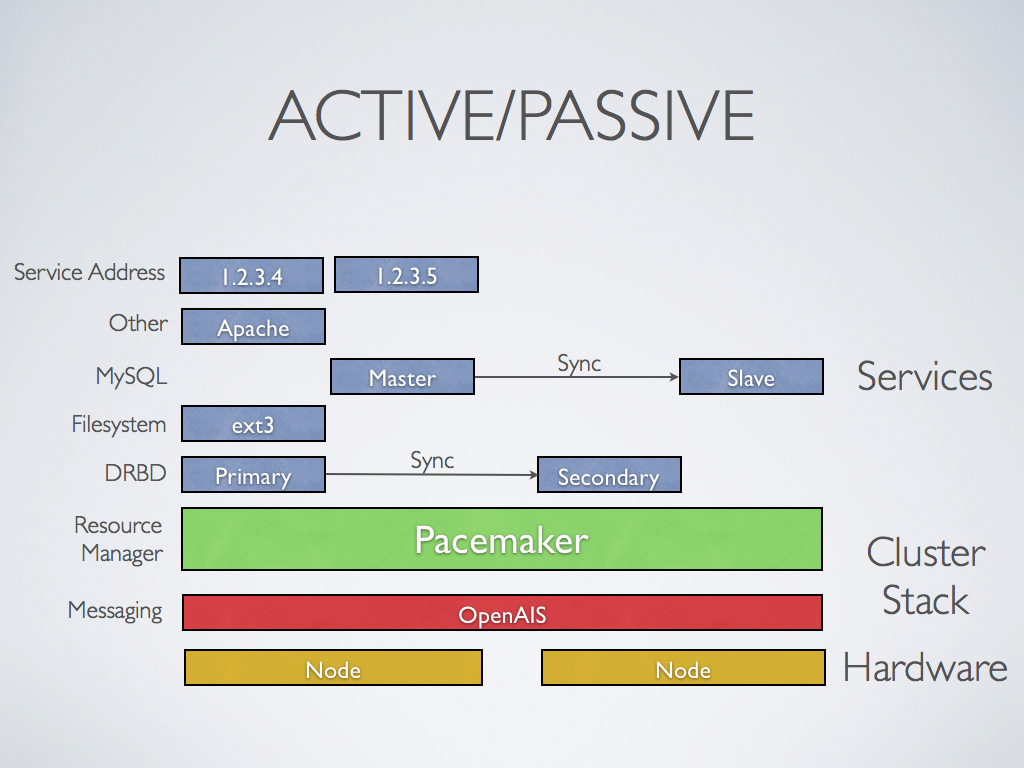
\includegraphics[keepaspectratio=true, width=\textwidth]{content/pacemaker-active-passive.png}\\[1cm]
                
                Les << node >> correspondent \`a nos machines (JB et LLM), la couche de messagerie OpenAIS correspondra au service Corosync qui est un projet d\'eriv\'e d'OpenAIS. Pour les couches sup\'erieures \`a Pacemaker, nous les avons vu pr\'ec\'edemment.\\
                
                Corosync est un moteur de clustering mettant en oeuvre une messagerie de service sur r\'eseau en utilisant une adresse et un port multicast.
                
            \subsection{Installation}
                
                \begin{bashcode}
                    # Installation de pacemaker et de corosync
                    yum install -y pacemaker corosync
                \end{bashcode}
                
            \subsection{Configuration}
                
                \subsubsection{Corosync}
                    
                    Avant toute chose, voici les adresses IP n\'ecessaires :\\
                    
                    \begin{description}
                        \item[Adresse IP multicast:] 239.0.0.1
                        \item[Port multicast:] 6800
                        \item[R\'eseau de la grappe:] 10.192.10.0
                        \item[Adresse IP de la grappe:] 10.192.10.50
                    \end{description}
                    
                    On va commencer par la configuration de Corosync qui est simpliste. Pour cela, on prends le fichier de configuration par d\'efaut et on va simplement y changer les adresses IP comme ceci :\\
                    
                    \begin{bashcode*}{gobble=24}
                        CONF="/etc/corosync/corosync.conf"
                        cp -f $CONF.example $CONF
                        sed -i.bak "s/.*mcastaddr:.*/mcastaddr:\ 239.0.0.1/g" $CONF
                        sed -i.bak "s/.*mcastport:.*/mcastport:\ 6800/g" $CONF
                        sed -i.bak "s/.*bindnetaddr:.*/bindnetaddr:\ 10.192.10.0/g" $CONF
                    \end{bashcode*}
                    
                    Ensuite, on va signaler \`a Corosync de charger le plugin Pacemaker afin qu'il puisse ''travailler'' avec :\\
                    
                    \begin{bashcode*}{gobble=24}
                        cat << EOT > /etc/corosync/service.d/pcmk
                        service {
                                # Load the Pacemaker Cluster Resource Manager
                                name: pacemaker
                                ver:  1
                        }
                        EOT
                    \end{bashcode*}
                    
                    Une fois configur\'e, nous pouvons lancer Corosync :\\
                    
                    \begin{bashcode*}{linenos=false, gobble=24}
                        /etc/init.d/corosync start
                    \end{bashcode*}
                    
                \subsubsection{Pacemaker}
                    
                    Pacemaker offre une invite de commande propre \`a lui-m\^eme (comme les switch Cisco) que nous pouvons lancer en tapant \verb+crm+. Il est int\'eressant de savoir qu'en interne, la configuration de Pacemaker est formatt\'ee en XML car suite \`a quelques erreurs de notre part, nous avons pu constater des erreurs de validation d'entr\'ee contre des Sch\'emas XML.\\
                    
                    Afin de vous \'epargner la configuration \`a la main de Pacemaker, nous pouvons exporter et injecter directement une configuration donn\'ee :\\
                    
                    \begin{bashcode*}{linenos=false, gobble=24}
                        crm configure load replace /path/to/conf/file
                    \end{bashcode*}
                    
                    Mais avant cela, vous devez d\'emarrer Pacemaker et vider sa configuration actuelle (si existante) :\\
                    
                    \begin{bashcode*}{linenos=false, gobble=24}
                        /etc/init.d/pacemaker start
                        cibsadmin -E --force
                    \end{bashcode*}
                    
                    Voici donc notre fichier de configuration pour Pacemaker (la version initiale qui marchait correctement) :\\
                    
                    \inputminted[
                        linenos,
                        bgcolor=lightgray,
                        tabsize=4,
                        fontfamily=courier,
                        fontsize=\small,
                        xleftmargin=5pt,
                        xrightmargin=5pt
                    ]{text}{./../confs/pcmk/conf.work}
                    
                    Dans ce fichier, on peut y entrevoir des d\'eclarations de ressources comme une IP ``flottante'' (\verb+10.192.10.50+) sur laquelle le monde ext\'erieur va se connecter au services que contient la grappe, des ressources de battement de coeurs pour un syst\`eme de fichier, les serveurs Apache, MySQL, LDAP et enfin la ressource de r\'eplication bas niveau DRBD.\\
                    
                    Mais ce n'est que la d\'eclaration des ressources, ensuite viennnent les d\'ependances de ``colocation'' qui obligent deux ressources donn\'ees \`a toujours \^etre de paire et enfin les ordres de d\'emarrage des ressources en fonction des d\'ependances.
                    Par exemple, Apache ne peut pas d\'emarrer avant que le syst\`eme de fichier soit op\'erationnel.
                    
                    Les autres fichiers de configuration sont disponibles en annexe \underline{\no\ref{pacemaker}}.
                    
                \subsection{Utilisation}
                    
                    Pour \st{admirer} surveiller le bon fonctionnement de Pacemaker, il y a la commande \verb+crm_mon+.\\
                    
                    En ce qui concerne la gestion des noeuds ou des ressources, il faut utiliser la commande \verb+crm+. Voici quelques exemples :\\
                    
                    \begin{bashcode*}{gobble=24}
                        # Verifier le status d'une ressource
                        crm resource status Apache
                        # Redemarrer une resource
                        crm resource restart MySQL
                        # Deplacer une ressource sur un autre noeud
                        crm ressource move FS mamba14
                        # Voir le status d'un noeud
                        crm node status mamba13
                        # Mettre un noeud en standby (simulation du failover)
                        crm node standby mamb14
                        # Et le rendre disponible a nouveau
                        crm node online mamba14
                    \end{bashcode*}
                    
    \part{Application Web}
        
        \section{Pr\'esentation}
            
            L'application Web demand\'ee devait permettre de d'afficher et d'ins\'erer des donn\'ees dans l'annuaire LDAP et dans la base de donn\'ees MySQL.\\
            
            D\'evelopp\'e en 3h seulement, l'application repose sur PHP 5.3 et utilise des frameworks r\'ecents comme \underline{\href{http://silex.sensiolabs.org}{Silex}} (\underline{\href{http://symfony.com}{Symfony 2}}), \underline{\href{http://framework.zend.com}{Zend Framework 2}} et enfin le framework CSS \underline{\href{http://twitter.github.com/bootstrap}{bootstrap}} de Twitter. Encore une fois, un maximum d'outils facile \`a mettre en oeuvre et puissants en quelques heures seulements.\\
            
            Une capture d'\'ecran de notre application est pr\'esente en annexe \underline{\no\ref{webapp}}.
            
        \section{Code source}
            
            Dans cette partie du rapport, nous allons vous montrer comment utiliser les outils choisis pour arriver \`a nos fins.
            
            \subsection{LDAP}
                
                Pour la partie LDAP, nous avons utilis\'e la \underline{\href{http://framework.zend.com/manual/fr/zend.ldap.html}{brique LDAP}} du Zend Framework 2.
                
                \subsubsection{Instance}
                
                    \begin{phpcode}
                        <?php
                        use Zend\Ldap\Ldap;
                        use Zend\Ldap\Exception as LdapException;
                        // ...
                        $app['ldap'] = $app->share(function() {
                            try {
                                $ldap = new Ldap(array(
                                    'host'              => 'ldap://localhost',
                                    'username'          => 'cn=manager,dc=g1b5,dc=tp,dc=org',
                                    'password'          => 'iamldapadmin',
                                    'bindRequiresDn'    => true,
                                    'accountDomainName' => 'g1b5.tp.org',
                                    'baseDn'            => 'ou=employee,dc=g1b5,dc=tp,dc=org',
                                ));
                                return $ldap->bind();
                            } catch (LdapException $e) {
                                var_dump($e->getMessage());
                            }
                        });
                    \end{phpcode}
                
                \subsubsection{R\'ecup\'eration de toute les personnes}
                
                    \begin{phpcode}
                        <?php
                        use Zend\Ldap\Ldap;
                        use Zend\Ldap\Exception as LdapException;
                        // ...
                        $app->get('/ldap.html', function(Silex\Application $app) {
                            $filter = Filter::equals('objectClass', 'person');
                            $results = $app['ldap']->search($filter, 'ou=employee,dc=g1b5,dc=tp,dc=org',
                            Ldap::SEARCH_SCOPE_SUB);
                            return $app['twig']->render('ldap.twig', array(
                                'dir'       => true,
                                'entries'   => $results
                            ));
                        });
                    \end{phpcode}
                    
                \subsubsection{Ajout d'une personne}
                    
                    \begin{phpcode}
                        <?php
                        use Zend\Ldap\Ldap;
                        use Zend\Ldap\Exception as LdapException;
                        // ...
                        $app->post('/ldap.html', function(Silex\Application $app) {
                            $name = $app->escape($app['request']->get('name'));
                            $entry = array();
                            Attribute::setAttribute($entry, 'cn', $name);
                            Attribute::setAttribute($entry, 'sn', $name);
                            Attribute::setAttribute($entry, 'objectClass', 'inetOrgPerson');
                            $app['ldap']->add('cn=' . $name . ' ,ou=employee,dc=g1b5,dc=tp,dc=org', $entry);
                            $filter = Filter::equals('objectClass', 'person');
                            $results = $app['ldap']->search($filter, 'ou=employee,dc=g1b5,dc=tp,dc=org',
                            Ldap::SEARCH_SCOPE_SUB);
                            return $app['twig']->render('ldap.twig', array(
                                'dir'       => true,
                                'entries'   => $results
                            ));
                        });
                    \end{phpcode}
            
            \subsection{MySQL}
                
                Concernant MySQL, nous n'avons pas utilis\'e d'ORM comme Doctrine mais nous avons simplement utilis\'e PDO.
                
                \subsubsection{Instance}
                    
                    \begin{phpcode}
                        <?php
                        $app['mysql'] = $app->share(function() {
                           try {
                               $pdo_options[\PDO::ATTR_ERRMODE] = \PDO::ERRMODE_EXCEPTION;
                               return new \PDO('mysql:host=localhost;dbname=projet_hd', 'root', 'pa$$wd',
                               $pdo_options);
                           } catch (\PDOException $e) {
                               var_dump($e->getMessage());
                           }
                        });
                    \end{phpcode}
                    
                \subsubsection{R\'ecup\'eration de tous les produits}
                    
                    \begin{phpcode}
                        <?php
                        $app->get('/mysql.html', function(Silex\Application $app) {
                            $response = $app['mysql']->query('SELECT * FROM `product`')
                                        ->fetchAll(\PDO::FETCH_ASSOC);
                            return $app['twig']->render('mysql.twig', array(
                                'db'        => true,
                                'entries'   => $response
                            ));
                        });
                    \end{phpcode}
                    
                \subsubsection{Ajout d'un produit}
                    
                    \begin{phpcode}
                        <?php
                        $app->post('/mysql.html', function(Silex\Application $app) {
                            $req = $app['mysql']->prepare('INSERT INTO product(name, price, quantity)
                                VALUES(:name, :price, :quantity)');
                            $req->execute(array(
                                'name'      => $app->escape($app['request']->get('name')),
                                'price'     => $app->escape($app['request']->get('price')),
                                'quantity'  => $app->escape($app['request']->get('qte'))
                            ));
                            $response = $app['mysql']->query('SELECT * FROM `product`')
                                        ->fetchAll(\PDO::FETCH_ASSOC);
                            return $app['twig']->render('mysql.twig', array(
                                'db'        => true,
                                'entries'   => $response
                            ));
                        });
                    \end{phpcode}
                    
    \part{Conclusion}
        \section{Difficult\'es rencontr\'es}
            
            Durant ce projet, la contrainte majeure \'etait de r\'ealiser une telle architechure en 3 jours seulement sans avoir aucune exp\'erience dans le domaine. Nous avons souhait\'e nous orienter vers des choix fonctionnels et matures plut\^ot qu'universitaires et peu professionnels.\\
            
            Le premier facteur de difficult\'e aura \'et\'e l'abscence d'indications concernant le choix des technologies car nous avons r\'eellement \'et\'e soumis \`a un environnement pragmatique o\`u nous jouons le r\^ole des responsables SI vers qui on vient se conseiller suite une probl\'ematique bien pr\'esente.
            Le choix et la d\'ecision des technologies est une chose mais ce qui est le plus chronophage est de regarder les produits et les solutions existantes sur le march\'e.\\
            
            Une fois les choix r\'ealis\'es, il a fallu se documenter pour savoir impl\'ementer au mieux possible l'infrastructure logicielle. Nous ne vous cacherons pas que nous avons lu 90\% de documentation en anglais durant ces 3 jours. De l'anglais pas toujours facile \`a comprendre de part ses termes techniques mais surtout de part la notion nouvelle que nous d\'ecouvrions sur le tas.\\
            
            La difficult\'e suivante fut li\'ee aux machines elles-m\^eme : impossible de pr\'evoir que tout va fonctionner du premier coup, le fait que les machines aient besoin d'un serveur mandataire pour acc\`eder au Web rajoute quelques contraintes sur les configurations mais surtout le manque de ma\^itrise complet sur les distributions Fedora nous aura fait perdre un peu de temps non n\'egligeable.\\
            
            Malgr\'e tout cela, nous sommes parvenus automatiser de mani\`ere relativement compl\`ete l'installation, la configuration et le d\'eploiement de notre projet \`a l'aide de Subversion et de scripts Bash.
            
        \section{Retours sur \'echec}
            
            Apr\`es 3 jours de recherche, de d\'eveloppement et de tests acharn\'es sur les diff\'erentes briques de notre architechure, nous avons \'echou\'e lors de la pr\'esentation de notre projet. En voici les raisons majeures :\\
            
            \begin{enumerate}
                \item Manque d'exp\'erience avec les technologies utilis\'ees
                \item Manque d'organisation et de rigueur dans les proc\'edures
                \item Manque de temps (implique du stress)
                \item Analyses sur tests d\'efaillants pas assez compl\`etes
            \end{enumerate}
            
            D'une certaine mani\`ere, tous ces facteurs sont li\'es car ils s'entre-croisent et s'encouragent et nous le savions mais pas c'est pas toujours \'evident d'avoir le temps de prendre le recul n\'ecessaire afin de mieux repartir.\\
            
            Apr\`es des heures intensives de travail, nous avions r\'eussi \`a faire tourner notre architechure active/passive en simulant des failovers et des failback avec succ\`es mais sans tester tous les cas possibles et surtout les cas d'\'evaluation. Suite \`a ce succ\`es pr\'ecipit\'e, nous avons voulu optimiser la configuration de Pacemaker afin de la simplifier mais nous nous sommes rendu compte apr\`es analyse que cette nouvelle configuration ne r\'epondait plus au contraintes d'ordre de basculement des services lors du failover.
            
            Dans le stress et la pr\'ecipitation, nous avons voulu essayer une architechure active/active car nous pensions que le type d'architechure active/passive ne r\'epondait pas \`a la demande de l'\'evaluation (analyse d'\'echec pas assez pouss\'ee) mais pr\`es quelques heures d'installation et de configuration, cette nouvelle monture n'a pas \'et\'e un succ\`es \`a cause d'un soucis de synchronisation de volume avec DRBD bien que la nouvelle configuration active/active de Pacemaker \'etait d\'ej\`a pr\`ete.
            
        \section{Retours personnels}
            
            \subsection{Joris \textsc{BERTHELOT}}
                
                Bien que le projet ne fut pas un succ\`es au moment de l'\'evaluation, nous pouvons tout de m\^eme avancer que notre architechure a bel et bien tourn\'e et surtout sous les yeux d'un de nos \'evaluateur quelques heures auparavant. C'est donc tout de m\^eme avec une certaine d\'eception que nous vous remettons ce dossier sachant que son contenu n'a pas pu fonctionner comme nous l'aurions souhait\'e au moment id\'eal.\\
                
                Tr\`es personnellement, j'ai \'eprouv\'e un r\'eel plaisir \`a m'activer intens\'ement pour la bonne r\'eussite du projet et m\^eme si nous n'avons pas r\'eussi, j'ai appris \'enorm\'ement de choses sur un domaine qui m'attirait depuis quelques temps d\'ej\`a. En PME ou en auto-entreprise, il est vraiment peu probable de devoir r\'ealiser de genre d'architechure en grappe donc je suis tr\`es agr\'eablement surpris d'avoir abord\'e cela en cycle universitaire.
                
            \subsection{Laurent \textsc{LE MOINE}}
                
                J'ai trouv\'e ce projet int\'eressant, et ancr\'e dans les probl\'ematiques propres aux entreprises, ce qui change par rapport aux projets habituels.\\
                
                L'installation des diff\'erents services ne nous \`a pos\'e de probl\`emes, \`a part LDAP qui ne prenait pas en compte le fichier de configuration et utilisait la nouvelle m\'ethode, mais une fois ceci compris nous n'avons pas eu d'autres probl\`emes.\\
                
                Les gros probl\`emes sont bien sur venus de DRBD et Pacemaker. Nous \'etions arriv\'es a une configuration relativement fonctionnelle et efficace, bien qu'elle n'\'etait pas parfaite. Le passage \`a la configuration Actif/Actif a \'et\'e une erreur.\\
                
                Avec le recul, nous aurions d'abord du pr\'eparer une r\'eplication basique, mais fonctionnelle, puis ensuite s'occuper de mettre en place DRBD et PaceMaker, plus efficaces et plus professionnels. Nous sommes partis sur le postulat que dans une entreprise il vaut mieux mettre en place ce genre de syst\`emes, plut\^ot que la r\'eplication basique de MySQL et de LDAP. Ces syst\`emes ont l'avantage de se g\'erer tous seuls.
                
                \vfill
                \flushright{Joris \textsc{BERTHELOT}\\
                joris@berthelot.tel\\
                \&\\
                Laurent \textsc{LE MOINE}
                \\laurent.le.moine17@gmail.com}
                \flushleft{}
                
    \appendix
    
    \part{Annexes}
        
        \section{Bind} \label{bind}
            
            Fichier de configuration du serveur esclave :\\
            
            \inputminted[
                linenos=true,
                bgcolor=lightgray,
                tabsize=4,
                fontfamily=courier,
                fontsize=\small,
                xleftmargin=5pt,
                xrightmargin=5pt
            ]{text}{./../confs/bind/named.conf.slave}
            
            Fichier de configuration de zone :\\
            
            \inputminted[
                linenos=true,
                bgcolor=lightgray,
                tabsize=4,
                fontfamily=courier,
                fontsize=\small,
                xleftmargin=5pt,
                xrightmargin=5pt
            ]{text}{./../confs/bind/g1b5.tp.org.zone}
            
            Fichier de configuration de zone inverse IPv4 :\\
            
            \inputminted[
                linenos=true,
                bgcolor=lightgray,
                tabsize=4,
                fontfamily=courier,
                fontsize=\small,
                xleftmargin=5pt,
                xrightmargin=5pt
            ]{text}{./../confs/bind/rv4.g1b5.tp.org.zone}
            
            Fichier de configuration de zone inverse IPv6 :\\
            
            \inputminted[
                linenos=true,
                bgcolor=lightgray,
                tabsize=4,
                fontfamily=courier,
                fontsize=\small,
                xleftmargin=5pt,
                xrightmargin=5pt
            ]{text}{./../confs/bind/rv6.g1b5.tp.org.zone}
            
        \section{Pacemaker} \label{pacemaker}
            
            Fichier de configuration de Pacemaker qui a voulu notre chute :
            
            \inputminted[
                linenos,
                bgcolor=lightgray,
                tabsize=4,
                fontfamily=courier,
                fontsize=\small,
                xleftmargin=5pt,
                xrightmargin=5pt
            ]{text}{./../confs/pcmk/conf.fail}
            
            Fichier de configuration de Pacemaker pour une architechure active/active (non test\'e) :
            
            \inputminted[
                linenos,
                bgcolor=lightgray,
                tabsize=4,
                fontfamily=courier,
                fontsize=\small,
                xleftmargin=5pt,
                xrightmargin=5pt
            ]{text}{./../confs/pcmk/conf.aa}
            
        \section{Application Web} \label{webapp}
            
            Capture d'\'ecran de la page d'accueil de notre application Web :\\
            
            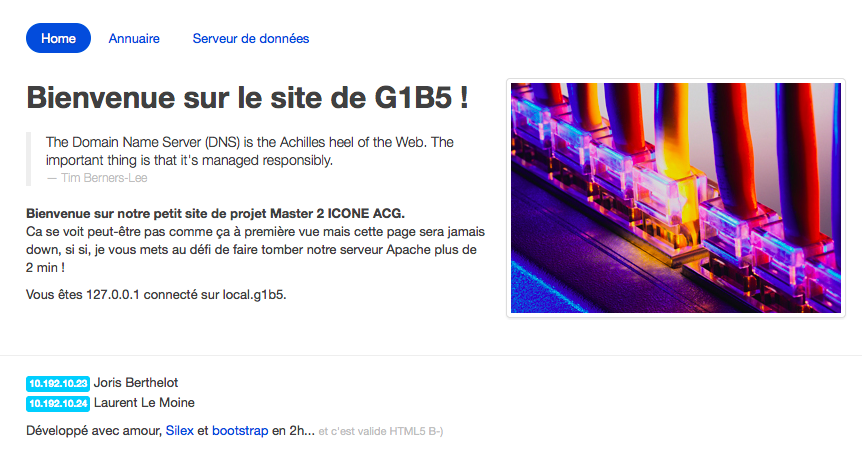
\includegraphics[keepaspectratio=true, width=\textwidth]{content/webapp_home.png}\\[1cm]
        
        \newpage
        
        \section{Bibliographie}
            
            Ici sont r\'epertori\'e tous les liens utiles pour l'avancement du projet.
            
            \subsection{LDAP}
                
                \url{http://www.openldap.org}
                \url{http://articles.mongueurs.net/magazines/linuxmag65.html}
                
            \subsection{MySQL}
                
                \url{http://dev.mysql.com/doc/refman/5.5/en/index.html}
                \url{}
                
            \subsection{Bind}
                
                \url{http://www.bind9.net/}
                \url{http://www.redfoxcenter.org/serveur/bind.html}
                
            \subsection{Pacemaker, DRBD}
                
                \url{http://www.clusterlabs.org/doc/en-US/Pacemaker/1.1/html/Clusters_from_Scratch/}
                \url{http://www.drbd.org/users-guide/re-drbdconf.html}
                \url{http://http://www.drbd.org/users-guide/re-drbdadm.html}
                \url{http://en.wikipedia.org/wiki/Computer_cluster}
                
\end{document}